\documentclass{article}
\usepackage[utf8]{inputenc}
\usepackage{graphics}
\title{Assignment1}
\author{Aditya Gangula EP20BTECH11001}

\begin{document}

\maketitle

\section*{Problem 3.20a}
Consider a causal LTI system implemented as the $RLC$ circuit shown in fig. \ref{prob}. In this circuit, $x(t)$ is the input voltage. The voltage $y(t)$ across the capacitor is considered the system output.
\begin{figure}[ht]
    \centering
    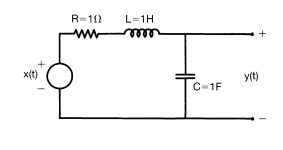
\includegraphics{probimg.png}
    \caption{3.20}
    \label{prob}
\end{figure}

\raggedright Find the differential equation relating $x(t)$ and $y(t)$.

\textbf {Solution:}

For the capacitor,
\[q = CV_c\]
\[ q = y(t)\]
Differentiating with time on both sides,
\[\frac{dq}{dt} = \frac{dy(t)}{dt}\]
Current flowing through the circuit is given by,
\[i = \frac{dy(t)}{dt}\]
Potential drop across the resistor is given by,
\[V_r = iR\]
\[V_r = \frac{dy(t)}{dt}\]
Potential drop across the inductor is given by,
\[V_l = L\frac{di}{dt}\]
\[V_l = \frac{d^2y(t)}{dt^2}\]
We have,
\[x(t) = V_r + V_l + V_c\]
\[x(t) = \frac{dy(t)}{dt}\ + \frac{d^2y(t)}{dt^2} + y(t)\]

\end{document}
